\documentclass{beamer}
\usepackage[spanish]{babel}
\usepackage[latin1]{inputenc}
\usepackage{multicol} % indice en 2 columnas
\usepackage{centernot}
\usepackage{amsmath}% http://ctan.org/pkg/amsmath

\usepackage{color}


\usepackage{graphicx}
\graphicspath{ {im/} }


\newcommand{\notimplies}{%
  \mathrel{{\ooalign{\hidewidth$\not\phantom{=}$\hidewidth\cr$\implies$}}}}


\usetheme{Warsaw}
%\usecolortheme{crane}
\useoutertheme{shadow}
\useinnertheme{rectangles}

\setbeamertemplate{navigation symbols}{} % quitar simbolitos



\title[Tema 2 - Vectores]{Vectores}
\subtitle{Estudios de Ingenier\'ia}
\author[https://frogames.es]{
Juan Gabriel Gomila%$^{1}$  \and E. Eva$^{2}$ \and S. Serpiente$^{3}$
}
\institute[Frogames]{
 % $^{1-2}$
 Frogames
   \and
  \texttt{https://frogames.es}
}
\date{\today}

\AtBeginSection{
\begin{frame}
  \begin{multicols}{2}
  \tableofcontents[currentsection]   
\end{multicols}
\end{frame}
}

\AtBeginSubsection{
\begin{frame}
  \begin{multicols}{2}
  \tableofcontents[currentsection,currentsubsection]
\end{multicols}
\end{frame}
}



%empieza aqui


\begin{document} 

\frame{\titlepage}

\begin{frame}
  \frametitle{\'Indice}
  \tableofcontents
\end{frame}

\section{Vectores}
\subsection{Definiciones}

\begin{frame}
  \frametitle{Vectores}
Los vectores tienen un papel fundamental no solo en matem\'aticas sino tambi\'en en la f\'isica, la ingenier\'ia e incluso otros campos cient\'ificos.

Ya se conocen de a\~nos anteriores las nociones de vectores en el plano o en el espacio. Los vectores en general tienen dos vertientes \'intimamente ligadas: la algebraica y la geom\'etrica.

Se ver\'a en primer lugar los vectores desde un punto de vista geom\'etrico.

\end{frame}



\begin{frame}
  \frametitle{Vectores}
  Sea $\mathbb{K}$ un cuerpo
  \begin{block}{Punto en la recta $\mathbb{K}$}
Dados un origen y una unidad de longitud, cada punto de la recta viene definido por un, y solo un, escalar del cuerpo $\mathbb{K}$ y viceversa.
  \end{block}

  \begin{block}{Punto en el plano $\mathbb{K}^2$}
Dados un origen, dos ejes (rectas) y una unidad de longitud, un punto del plano es un par $(x,y)$ donde $x$ y $y$ son dos elementos del cos $\mathbb{K}$.
  \end{block}
\end{frame}
  

\begin{frame}
  \frametitle{Vectores}
  \begin{block}{Punto en el espacio $\mathbb{K}^3$}
Dados un origen, tres ejes (rectas) y una unidad de longitud, un punto del plano es una terna $(x,y,z)$ donde $x,y$ y $z$ son dos elementos del cuerpo $\mathbb{K}$.
  \end{block}
\end{frame}


\begin{frame}
  \frametitle{Vectores}
  \begin{block}{Puntos en $\mathbb{K}^n$}
Un punto del espacio $\mathbb{R}^n$ se define como una $n$-tupla de n\'umeros:
\[X=(x_1,x_2,\cdots,x_n)\]
Donde $n$ es la dimensi\'on del espacio $\mathbb{K}^n$.
  \end{block}

  \begin{block}{Coordenadas del punto}
Las coordenadas de $X$ son los valores $x_1,x_2,\cdots, x_n$ del punto $X$.
  \end{block}

\end{frame}

\subsection{Vectores fijos}

\begin{frame}
  \frametitle{Vectores fijos}
Las siguientes definiciones permiten ver los vectores desde una perspectiva geom\'etrica:
  \begin{block}{Vector fijo}
Un vector fijo es un par de puntos $A$ y $B$, que se indicar\'an como $\vec{AB}$. El punto $A$ se denomina \textbf{origen} y el punto $B$ \textbf{extremo}.
  \end{block}

Normalmente los vectores en el plano o en el espacio de tres dimensiones se suelen representar mediante segmentos acabados en una punta de flecha en uno de sus dos extremos.
  
\end{frame}

Las componentes cartesianas de un vector son los vectores que se obtienen al proyectarlo sobre los ejes de un sistema de coordenadas situado en el origen del vector.


\begin{frame}
  \frametitle{Componentes de un vector fijo $\vec{AB}$ }
  \begin{block}{Vector fijo}
Las componentes de un vector fijo $\vec{AB}$ son los vectores que se obtienen al proyectarlo sobre los ejes de un sistema de coordenadas situado sobre el origen del vector.
\end{block}



\begin{figure}[h]
\caption{Criterio de colores. {\color{red}Rojo}:+ {\color{green}Verde}:-. Las  componentes pueden ser positivas o negativas}
    \label{fig:vectores}
\centering
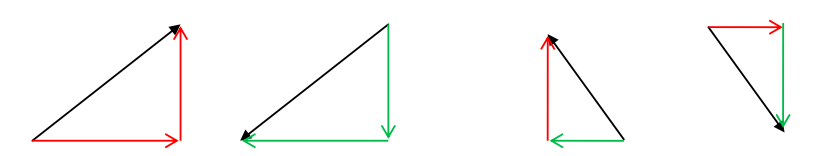
\includegraphics[width=\textwidth]{vectors}
\end{figure}


\end{frame}

\begin{frame}
  \frametitle{Vectores fijos}
  \begin{block}{Componentes de un vector fijo $\vec{AB}$}
Si $A=(a_x,a_y)$ y $B=(b_x,b_y)$ entonces las componentes del vector $\vec{AB}$ se obtienen restando las coordenadas del punto extremo $B$ al punto de origen $A$:
\[\vec{AB} = (b_x-a_x, b_y-a_y)\]
  \end{block}
\end{frame}




\begin{frame}
  \frametitle{Vectores fijos}
  El valor absoluto de las componentes del vector coincide con la de los catetos del tri\'angulo rect\'angulo formado y tal que el vector sea su hipotenusa. 
  
  
\begin{figure}[h]
    \label{fig:componentes}
\centering
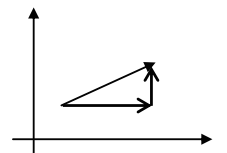
\includegraphics[scale=0.5]{components}
\end{figure}


\end{frame}




\begin{frame}
  \frametitle{Vectores fijos}

  
\begin{figure}[h]
    \label{fig:ejemplo de componentes}
\centering
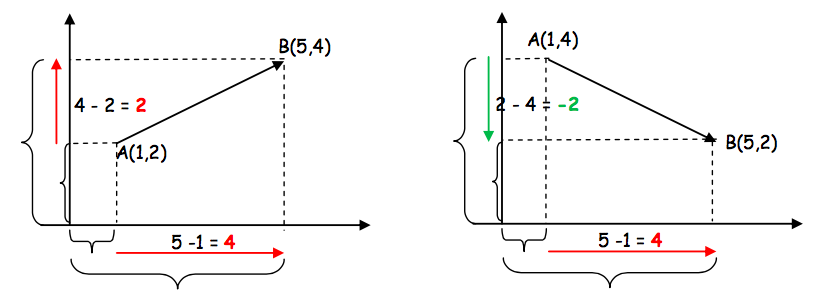
\includegraphics[width=\textwidth]{components_example}
\end{figure}


\end{frame}




\begin{frame}
  \frametitle{Vectores fijos}
  \begin{block}{Caracterizaci\'on de un vector fijo (I)}
En el contexto geom\'etrico, las 3 caracter\'isticas de un vector fijo son:
\begin{itemize}
\item Origen: el punto de aplicaci\'on donde comienza el vector
\item M\'odulo: la longitud del segmento
\item Direcci\'on: la de la recta a la cual pertenece
\item Sentido: el que determina la punta de la flecha del vector
\end{itemize}
\end{block}
\end{frame}

\begin{frame}
  \frametitle{Vectores fijos}
  \begin{block}{Caracterizaci\'on de un vector fijo (II)}
Tambi\'en queda completamente determinado con:
\begin{itemize}
\item Sus componentes
\item El punto origen
\end{itemize}
\end{block}
\end{frame}

\begin{frame}
  \frametitle{Vectores fijos}
  \begin{block}{Caracterizaci\'on de un vector fijo (III)}
O incluso si se conocen:
\begin{itemize}
\item Las coordenadas del punto origen
\item Las coordenadas del punto extremo
\end{itemize}
\end{block}
\end{frame}





\begin{frame}
  \frametitle{Vectores equivalentes}
  \begin{block}{Vectores equivalentes}
Dos vectores $\vec{AB}$ y $\vec{CD}$ son equivalentes si tienen las mismas componentes; es decir:
\[(b_x-a_x,b_y-a_y) = (d_x-c_x,d_y-c_y)\]
\end{block}
\end{frame}


\begin{frame}
  \frametitle{Vectores equivalentes}
\begin{figure}[h]
    \label{fig:vectores equivalentes}
\centering
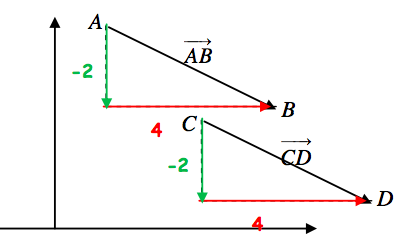
\includegraphics[scale=0.2]{vectors_equivalents}
\caption{$\vec{AB}$ y $\vec{CD}$ son equivalentes incluso al tener diferentes or\'igenes y extremos}

\end{figure}

Geom\'etricamente, las longitudes de los segmentos de la recta determinados por el par de puntos y los sentidos de ambos vectores son iguales.
\end{frame}


\begin{frame}
  \frametitle{Vectores equivalentes}
  \begin{block}{Ejercicios}
Encu\'entrese un vector equivalente a $\vec{AB}$ donde $A=(1,2)$ y $B=(5,4)$
\end{block}
Sol: Puntos cualesquiera $C$ y $D$ tales que:
\[(d_x-c_x,d_y-c_y) = (4,2)\]
\end{frame}

\begin{frame}
  \frametitle{Vectores equivalentes}
  \begin{block}{Ejercicios}
Encu\'entrese un vector equivalente a $\vec{AB}$ donde $A=(3,4)$ y $B=(7,6)$ con origen en el punto $A=(-1,0)$.
\end{block}
Sol: 
\[B'=(3,2)\]
\end{frame}




\subsection{Vectores libres}
\begin{frame}
  \frametitle{Vectores libres}

Todos los vectores fijos equivalentes entre s\'i tienen las mismas componentes. En este sentido es posible establecer una relaci\'on de equivalencia correspondiente, el \textbf{vector libre}. Estre representante define un conjunto infinito de vectores y los representa a todos ellos.


\end{frame}




\begin{frame}
  \frametitle{Vectores libres}


  \begin{block}{Vectores libres}
El conjunto de todos los vectores fijos equivalentes entre s\'i se denomina vector libre. Un vector libre no tiene un origen fijo, sino que se puede ubicar en cualquier punto del espacio. Cada vector fijo es un representante del vector libre.
\end{block}

\begin{figure}[h]
    \label{fig:vector libre}
\centering
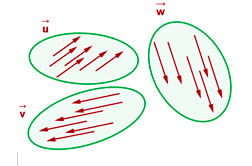
\includegraphics[scale = 0.6]{vector_lliure}
\end{figure}

\end{frame}


\begin{frame}
  \frametitle{Vectores libres}
  \begin{block}{Vector fijo en el origen}
Es aquel de los representantes del vector fijo que tienen su punto origen en el origen de coordenadas.
\end{block}
En este caso, las coordenadas del punto extremo coinciden num\'ericamente con las componentes del vector, ya que el punto de origen es $0=(0,0)$.
\begin{figure}[h]
    \label{fig:vector libre en el origen}
\centering
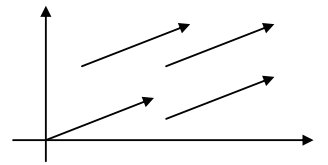
\includegraphics[scale = 0.6]{vec_lliure_origin}
\end{figure}

\end{frame}


\begin{frame}
  \frametitle{Vectores libres}
  
  Por tanto, todo vector libre tiene un representante situado en el origen de coordenadas donde el punto extremo tiene las mismas coordenadas que las componentes del vector. En este sentido se puede decir:
  \begin{block}{Resultado}
Existe una correspondencia uno a uno entre los vectores libres y los puntos seg\'un el cual cada punto $P=(a,b)$ se identifica con un vector $\vec{OP} = (a,b)$.
 \end{block}
\end{frame}



\begin{frame}
  \frametitle{Vectores libres}
  
  \begin{block}{Caracteritzaci\'on de un vector libre (I)}
Para caracterizar un vector libre se necesitar\'a el m\'odulo, la direcci\'on y el sentido.
 \end{block}
   \begin{block}{Caracteritzaci\'on de un vector libre (II)}
Tambi\'en se puede caracterizar si se conocen las componentes
\end{block}
El m\'odulo, al igual que en los vectores fijos, viene dado por la longitud del segmento y la direcci\'on y sentido vienen definidos por el \'angulo que forma el vector con la direcci\'on positiva del eje $OX$..

\end{frame}

\begin{frame}
  \frametitle{Vectores libres}
  
  \begin{block}{Ejercicios}
Encu\'entrse el m\'odulo, direcci\'on y sentido del vector de componentes (7,-5). 
\end{block}
Sol: m\'odulo $=\sqrt{74}$ y $\tan \alpha=\frac{-5}{7}$
   \begin{block}{Ejercicios}
  Dado el vector de m\'odulo $8$ y el hecho de que forma un \'angulo de $135$ grados con el eje $OX$, calc\'ulense sus componentes.
    \end{block}
Sol:$(8\cos 135, 8\sin 135)$
\end{frame}


\section{Operaciones con vectores}

\subsection{Suma y resta de vectores libres}

\begin{frame}
  \frametitle{Suma de vectores libres}
  
  \begin{block}{Definici\'on}
Sea $\vec{u} = (u_1,u_2, \cdots, u_n)$ y $\vec{v} = (v_1,v_2,\cdots,v_n)$, entonces:
\[\vec{u}+\vec{v} = (u_1+v_1, u_2+v_2, \cdots, u_n+v_n)\]
\end{block}
Geom\'etricamente es el vector formado por la diagonal del paralelogramo que tiene los dos vectores sumandos como lados y origen el mismo que ambos.
\begin{figure}[h]
    \label{fig:suma}
\centering
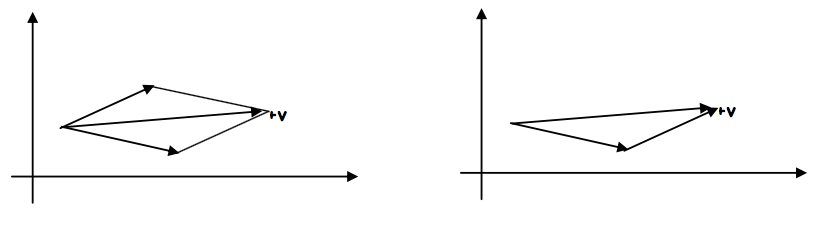
\includegraphics[width = \textwidth]{suma}
\end{figure}
\end{frame}


\begin{frame}
  \frametitle{Suma de vectores libres}
  

Si se han de sumar m\'as de dos vectores, resulta m\'as \'util la segunda construcci\'on gr\'afica. Basta colocar cada origen de los vectores sumandos sobre el extremo del vector sumando precedente
 \begin{figure}[h]
    \label{fig:suma}
\centering
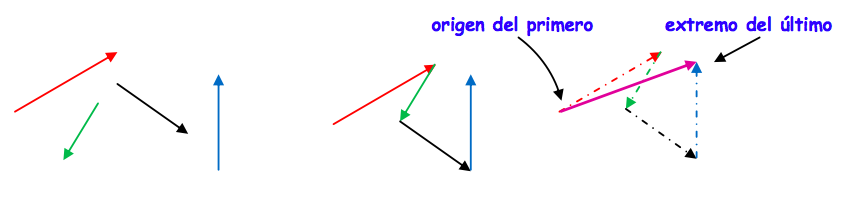
\includegraphics[width = \textwidth]{suma_2}
\end{figure}
\end{frame}






\begin{frame}
  \frametitle{Resta de vectores libres}
  
  \begin{block}{Definici\'on}
Sea $\vec{u} = (u_1,u_2, \cdots, u_n)$ y $\vec{v} = (v_1,v_2,\cdots,v_n)$, entonces
\[\vec{u}-\vec{v} = (u_1-v_1, u_2-v_2, \cdots, u_n-v_n)\]
\end{block}
Geom\'etricamente se realiza la suma entre el vector minuendo y el opuesto del sustraendo.
\begin{figure}[h]
    \label{fig:resta}
\centering
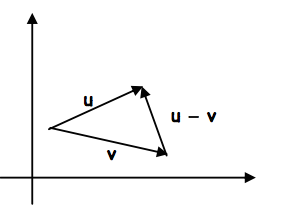
\includegraphics[width = 5cm]{resta}
\end{figure}
\end{frame}


\begin{frame}
  \frametitle{Resta de vectores libres}
  

Una peque\~na observaci\'on: al realizar la resta $\vec{u} - \vec{v}$ se busca un vector $\vec{w}$ tal que si se le suma al sustraendo ha de dar el minuendo:
\begin{figure}[h]
    \label{fig:resta}
\centering
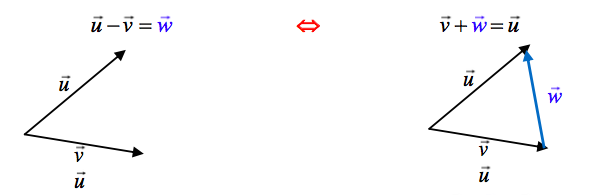
\includegraphics[width = \textwidth]{resta_2}
\end{figure}
\end{frame}


\begin{frame}
  \frametitle{Obtenci\'on de las componentes de un vector $\vec{AB}$}
  

Si se tiene un vector $\vec{AB}$ obtenido a partir de los puntos $A$ y $B$ y se dibujan los vectores $\vec{OA}$ y $\vec{OB}$
\begin{figure}[h]
    \label{fig:componentes de la suma}
\centering
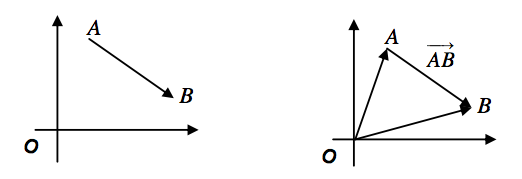
\includegraphics[width = \textwidth]{components_suma}
\end{figure}
Entonces se puede ver como $\vec{AB}$, $\vec{OA}$ y $\vec{OB}$ forman un tri\'angulo vectorial y se pueden escribir las relaciones siguientes:
\[\vec{OA}+\vec{AB}-\vec{OB} = \vec{0}\Rightarrow \vec{AB} = \vec{OB}-\vec{OA}\]
\end{frame}




\begin{frame}
  \frametitle{Obtenci\'on de las componentes de un vector $\vec{AB}$}
  
  \begin{block}{Ejercicios}
Obt\'engase $\vec{SR}$ a partir de $\vec{OR} = (-1,4)$ i $\vec{OS} = (-3,-2)$
\end{block}

  \begin{block}{Ejercicios}
Obt\'engase $\vec{PR}-\vec{PS}$ a partir de $\vec{OR} = (-1,4)$, $\vec{OS} = (-3,-2)$ i $\vec{OP} = (3,0)$.
\end{block}

\end{frame}





\begin{frame}
  \frametitle{Obtenci\'on de las componentes de un vector $\vec{AB}$}
  

\begin{figure}[h]
    \label{fig:ejemplo sobre componentes}
\centering
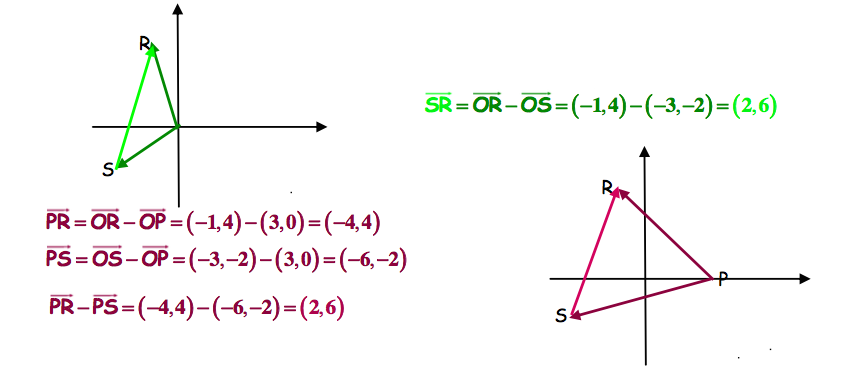
\includegraphics[width = \textwidth]{ex_components}
\end{figure}
\end{frame}



\subsection{Producto de vector por escalar}

\begin{frame}
  \frametitle{Producto por escalar}
  
  \begin{block}{Definici\'on}
Sea $\vec{u} = (u_1,u_2,\cdots,u_n)\in\mathbb{K}^n$ y sea $\lambda\in\mathbb{K}$ entonces:
\[\lambda\vec{u} =  (\lambda u_1, \lambda u_2,\cdots, \lambda u_n)\in\mathbb{K}^n \]
\end{block}

\begin{figure}[h]
    \label{fig:componentes del producto}
\centering
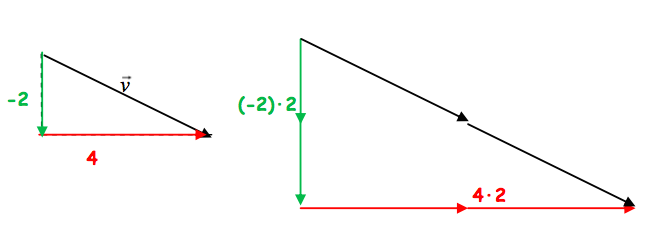
\includegraphics[width = \textwidth]{components_product}
\end{figure}

\end{frame}

\begin{frame}
  \frametitle{Producto por escalar}
 
 En el ejemplo anterior $\vec{v} = (4,-2)$ y $2\vec{v} = (8,-4)$. Adem\'as, la longitud de $\vec{v} = 2\sqrt{5} $ y la de $2\vec{v} = 4\sqrt{5}$, donde se observa que al duplicar el vector, tambi\'en se duplica su m\'odulo o longitud. En cambio la direcci\'on y sentido de $\vec{2v}$ coincide con la de $\vec{v}$. Se ver\'a que no siempre ser\'a as\'i.
\end{frame}


\begin{frame}
  \frametitle{Producto por escalar}
 
El resultado de multiplicar un escalar $\lambda\neq 0 $ por un vector $\vec{v}$ es otro vector $\vec{u}$ de la mismas direcci\'on que $\vec{v}$, de sentido igual o contrario seg\'un sea el signo del escalar $+$ o $-$, y de m\'odulo igual a $\lambda$ veces el de $\vec{v}$
\begin{figure}[h]
    \label{fig:producto por escalar}
\centering
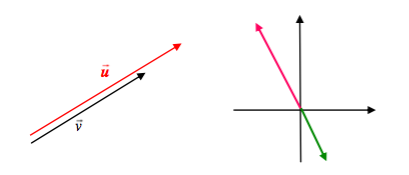
\includegraphics[height = 3cm]{pte_escalar}
\caption{A la figura de la derecha, si el vector $\vec{v}=(1,-2)$ se multiplica por el escalar $-2$ se obtiene otro vector $\vec{u}$ paralelo a $\vec{v}$ y de componente $\vec{u} = (-2,4)$.}
\end{figure}

\end{frame}


\begin{frame}
  \frametitle{Producto por escalar}
  
  \begin{block}{Vectores paralelos}
Dos vectores $\vec{u} =(u_1,u_2,\cdots,u_n)$ y $\vec{v}=(v_1,v_2,\cdots,v_n)$ son paralelos (o proporcionales) si existe un valor $\lambda\neq 0$ tal que $\vec{u} = \lambda \vec{v}$. \end{block}
Ser\'an del mismo sentido si $\lambda>0$ y de sentidos opuestos si $\lambda<0$.

\end{frame}


\begin{frame}
  \frametitle{Producto por escalar}
  
  \begin{block}{Ejercicios}
Dados los puntos $A=(1,2,3), B=(0,-1,2)$ y $C=(-2,-7,0)$, si $D$ es el punto de coordenadas $(-1,x,0)$ encu\'entrese, si es posible, el valor de $x$ para el que los vectores $\vec{AB}$ y $\vec{CD}$ son paralelos. Raz\'onese el procedimiento empleado.
\end{block}
Sol: el problema no tiene soluci\'on.
\end{frame}


\begin{frame}
  \frametitle{Producto por escalar}
  
  \begin{block}{Ejercicios}
Dados los vectores $\vec{u}=(2,3,0)$ y $\vec{v}=(-3,0,1)$ encu\'entrese el valor de $k$ para el que los vectores $\vec{a}$ y $\vec{b}$ son paralelos, donde $\vec{a} = 2\vec{u}-\vec{v}$ y $\vec{b} = -3\vec{u}+k\vec{v}$.
\end{block}
Sol: $k = \frac{3}{2}$.
\end{frame}

\subsection{Combinaci\'on lineal de vectores}
\begin{frame}
  \frametitle{Combinaci\'on lineal}
  
  \begin{block}{Combinaci\'on lineal de vectores}
Dados $V = \{\vec{v_1},\vec{v_2},\cdots,\vec{v_k}\}$ un conjunto de vectores de $\mathbb{K}^n$ y $\alpha_1,\alpha_2,\cdots,\alpha_k \in \mathbb{K}$ se define la combinaci\'on lineal de los vectores de $V$ como el vector $\vec{w}$:
\[\vec{w} = \alpha_1\vec{v_1}+\alpha_2\vec{v_2}+\cdots+\alpha_k\vec{v_k} =\sum_{i=1}^{k}\alpha_i\vec{v_i} \]
\end{block}
La combinaci\'on lineal de vectores no es una operaci\'on nueva, sino que reune en un mismo lugar la suma de vectores y el producto por escalares. Para poder hacer combinaciones lineales de vectores es necesario que todos ellos tengan el mismo n\'umero de componentes y el resultado ser\'a otro vector de estas mismas caracter\'isticas.
\end{frame}

\begin{frame}
  \frametitle{Combinaci\'on lineal}
    \begin{block}{Ejercicios}
?`Es el vector $(2,3)$ combinaci\'on lineal de $(3,1)$ y $(-6,-2)$? Justif\'iquese gr\'aficamente la respuesta.
\end{block}
Sol: no.
\end{frame}


\section{Propiedades de las operaciones con vectores}
\begin{frame}
  \frametitle{Propiedades de las operaciones con vectores}
  Al definir las operaciones de suma y producto por un escalar conviene tener presentes las diferencias y similitudes entre ambos.
    \begin{block}{Ley de composici\'on interna}
La suma de vectores se denomina ley de composici\'on interna ya que opera entre elementos de un conjunto dado, $\mathbb{K}^n$ y el resultado es otro elemento de este conjunto:
\[\begin{array}{r@{\hspace{-2pt}}c@{\hspace{-4pt}}
c@{\hspace{4pt}}l}
f:&\mathbb K^n\times \mathbb K^n&\longrightarrow&\mathbb K^n\\
  &(\vec{u}, \vec{v})\ \ &\mapsto&\vec u + \vec v
\end{array}\]
\end{block}
\end{frame}

\begin{frame}
  \frametitle{Propiedades de las operaciones con vectores}
    \begin{block}{Ley de composici\'on externa}
El producto de un escalar por un vector tiene como operandos conjuntos diferentes: escalares por un lado y vectores por el otro. El resultado cae del lado de los vectores, y la operaci\'on se denomina ley de composici\'on externa:
\[\begin{array}{r@{\hspace{-2pt}}c@{\hspace{-4pt}}
c@{\hspace{4pt}}l}
f:&\mathbb K\times \mathbb K^n&\longrightarrow&\mathbb K^n\\
  &(\lambda, \vec{v})\ \ &\mapsto&\lambda  \vec v
\end{array}\]
\end{block}
\end{frame}



\begin{frame}
  \frametitle{Propiedades de la suma de vectores}
Sea $\vec u, \vec v, \vec w\in \mathbb K^n$ y $\alpha, \beta\in\mathbb K$ entonces se cumple:
    \begin{block}{Propiedades}
\begin{itemize}
\item Ley asociativa: $(\vec u+\vec v) +\vec w = \vec u +(\vec v + \vec w)$
\item Ley conmutativa: $\vec u+\vec v = \vec v +\vec u$
\item Elemento neutro de la suma: $\vec u+\vec 0 = \vec 0 +\vec u = \vec u$
\item Vector opuesto: $\vec u+(-\vec{u}) = (-\vec u) +\vec u = \vec 0$
\end{itemize}
\end{block}
\end{frame}

\begin{frame}
  \frametitle{Propiedades del producto por un escalar}
    \begin{block}{Propiedades}
\begin{itemize}
\item Ley distributiva del producto por un escalar para la suma de vectores: $\alpha(\vec u+\vec v)  = \alpha\vec u +\alpha\vec v $
\item Ley distributiva del producto de un vector por la suma de escalares: $(\alpha+\beta)\vec u =\alpha \vec u +\beta\vec u$
\item Ley asociativa del producto entre escalares y vectores: $(\alpha\beta)\vec u = \alpha (\beta\vec u) = \beta(\alpha\vec u )$
\item Elemento unidad: $1\vec u = \vec u$
\end{itemize}
\end{block}
\end{frame}


\section{Estructura euclidiana de $\mathbb{R}^n$}

\subsection{Producto escalar}

\begin{frame}
  \frametitle{Producto Escalar}
El producto escalar es la tercera operaci\'on b\'asica entre vectores de $\mathbb R^n$. 
    \begin{block}{Producto escalar}
    Sean $\vec u = (u_1,u_2,\cdots,u_n)$ y $\vec{v} = (v_1,v_2,\cdots,v_n)$ dos vectores de $\mathbb R^n$. Se define el producto escalar $\vec u \cdot \vec v$ como el n\'umero real
    \[\vec u \cdot \vec v = u_1v_1+u_2v_2+\cdots+u_nv_n\]
\end{block}
De ello se derivan los conceptos m\'etricos como la ortogonalidad, la norma, el \'angulo y se abre camino a m\'ultiples aplicaciones geom\'etricas y f\'isicas del \'algebra lineal. 
\end{frame}


\begin{frame}
  \frametitle{Producto escalar}
    \begin{block}{Ejemplo}
    Sean $\vec u = (2,3,0)$ y $\vec{v} = (-1,-3,1)$ dos vectores de $\mathbb R^3$. Calc\'ulese su producto escalar:
\end{block}
Sol:    \[\vec u \cdot \vec v = -11\]
\end{frame}


\begin{frame}
  \frametitle{Propiedades del producto escalar}
    \begin{block}{Propiedades}
\begin{itemize}
\item Conmutativa: $\vec u\cdot \vec v = \vec v \cdot \vec u $
\item Distributiva respecto de la suma: $\vec v \cdot (\vec u + \vec w) = \vec v\cdot \vec u + \vec v \cdot \vec w$
\item Asociativa y conmutativa entre escalares y vectores: 
\[(\lambda\vec u) \cdot \vec v = \lambda (\vec u \cdot \vec v)\]
\[\vec u\cdot (\lambda \vec v) = \lambda (\vec u \cdot \vec v)\]
\item Si $\vec u = \vec 0 \Rightarrow \vec u \cdot \vec u = 0$. 
\item Si $\vec u \neq \vec 0 \Rightarrow \vec u \cdot \vec u > 0$.
\end{itemize}
\end{block}
\end{frame}

\begin{frame}
  \frametitle{Propiedades del producto escalar}
    \begin{block}{Ejercicios}
Dados los vectores $\vec u = (2,-1,5), \vec v = (-3,4,1)$ y $\vec w = (-1,0,5)$
\begin{enumerate}
\item Compru\'ebese que el producto escalar tiene la propiedad conmutativa.
\item Compru\'ebese que el producto escalar tiene la propiedad distributiva respecto de la suma.
\item Compru\'ebese que el producto escalar tiene la propiedad asociativa entre escalares y vectores.
\end{enumerate}
\end{block}
\end{frame}

\begin{frame}
  \frametitle{Propiedades del producto escalar}
    \begin{block}{Ejercicios}
Demu\'estrese que si $\vec u \neq \vec 0$ entonces $\vec u \cdot \vec u >0$
\end{block}
\end{frame}


\subsection{Norma o longitud}

\begin{frame}
  \frametitle{Norma de un vector}
    \begin{block}{Norma}
Dado $\vec u = (u_1,u_2\cdots,u_n)\in \mathbb R^n$ su norma o longitud viene dada por:
\[||\vec u || = \sqrt{\vec u \cdot \vec u} = \sqrt{u_1^2+u_2^2+\cdots+u_n^2}\]
\end{block}
En muchos casos resulta \'util la norma al cuadrado de un vector:
\[||\vec u||^2 = ( \sqrt{\vec u \cdot \vec u})^2 \Rightarrow ||\vec u||^2 = \vec u \cdot \vec u \]
\end{frame}


\begin{frame}
  \frametitle{Norma de un vector}
    \begin{block}{Ejercicios}
Dado $\vec u = (2,3,-1)\in \mathbb R^3$, calc\'ulese su longitud.
\end{block}
Sol: \[||\vec u|| = \sqrt{14} \]
\end{frame}

\begin{frame}
  \frametitle{Norma de un vector}
    \begin{block}{Propiedades}
\begin{itemize}
\item $||\vec u||>0, \forall \vec u \neq \vec 0$
\item $||\lambda \vec u|| = |\lambda|.||\vec u||$
\item $|| \vec u+\vec v|| \leq ||\vec u||+||\vec v||$ (Desigualdad triangular)
\item $|| \vec u+\vec v|| = ||\vec u||+||\vec v||\Leftrightarrow \vec u \perp \vec v$ (teorema de Pit\'agoras)
\item $|| \vec u\cdot\vec v|| \leq ||\vec u||\cdot||\vec v||$ (Desigualdad de Cauchy-Schwarz)
\end{itemize}
\end{block}
\end{frame}

\begin{frame}
  \frametitle{Norma de un vector}
    \begin{block}{Ejercicios}
 Dado $\vec u = (2,3,-1)$ compru\'ebese que: 
 \[||2\vec u|| = 2||\vec u ||\]
 \[||-2\vec u|| = |-2|||\vec u || = 2||\vec u||\]
 \end{block}
\end{frame}

\begin{frame}
  \frametitle{Norma de un vector}
    \begin{block}{Vector unitario}
Un vector unitario $\vec e$ es aquel que tiene la norma 1: \[||\vec e|| = 1\]
 \end{block}
 Por ejemplo el vector $(1,0,0)$ es un vector unitario. 
\end{frame}


\begin{frame}
  \frametitle{Norma de un vector}
    \begin{block}{Ejercicios}
Dado el vector $\vec u = (2,3,-1)$ compru\'ebese que si se divide por su norma se obtiene otro vector que es unitario.
 \end{block}
     \begin{block}{Ejercicios}
Demu\'estrese que cualquiera que sea el vector $\vec u$, al ser dividido por su norma es unitario. 
\end{block}
    \begin{block}{Ejercicios}
Dado el vector $\vec u = (2,3,-1)$ encu\'entrese otro vector de la misma direcci\'on y sentido pero de norma igual a 3.
 \end{block}
 
\end{frame}



\subsection{Distancia entre dos puntos}


\begin{frame}
  \frametitle{Distancia entre dos puntos}
    \begin{block}{Distancia entre dos puntos}
Dados dos puntos $A$ y $B$ se define la distancia entre ambos como:
\[d(A,B) = ||\vec{AB}|| = \sqrt{\vec{AB}\cdot\vec{AB}}\]
 \end{block}
Este valor coincide con la intuici\'on geom\'etrica cuando $A$ y $B$ son dos puntos del plano. Equivale a la longitud del vector fijo $\vec{AB}$.

    \begin{block}{Ejercicios}
Dados dos puntos $A=(1,2)$ y $B=(4,3)$ encuentra la distancia entre ambos.
 \end{block}
 Sol: $\sqrt{10}$.
\end{frame}

\begin{frame}
  \frametitle{Distancia entre dos puntos}
    \begin{block}{Teorema}
Dados dos vectores $\vec u$ y $\vec v$  y $\alpha$ el \'angulo que forman ambos, entonces se cumple que:

\[\vec u \cdot \vec v = ||\vec u ||\cdot ||\vec v||\cdot  \cos \alpha\]
 \end{block}

\begin{figure}[h]
    \label{fig:teorema del coseno}
\centering
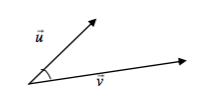
\includegraphics[height=3cm]{th_cos}
\end{figure}
\end{frame}

\begin{frame}
  \frametitle{Distancia entre dos puntos}
  Para hacer la demostraci\'on se utilizar\'a un resultado previo.
    \begin{block}{Teorema del coseno}
En un tri\'angulo $ABC$ cualquiera y siendo $\alpha,\beta,\gamma$ los \'angulos, y $a,b,c$ los \'angulos de los lados opuestos a los anteriores, entonces:

\[b^2=a^2+c^2-2ac\cos\alpha\]
 \end{block}

\begin{figure}[h]
    \label{fig:triangulo}
\centering
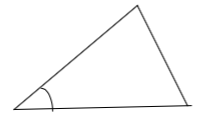
\includegraphics[height=3cm]{triangle}
\end{figure}
\end{frame}

\begin{frame}
  \frametitle{Distancia entre dos puntos}
    \begin{block}{Demostraci\'on}
En primer lugar se dibuja el vector $\vec u -\vec v$ con lo que queda dibujado un tri\'angulo. Se aplica la definici\'on de norma bajo la forma $||\vec w||^2 = \vec w \cdot \vec w$ al vector $\vec u -\vec v$, resulta:
\[||\vec u - \vec v||^2 = ||\vec u||^2+||\vec v||^2-2(\vec u\cdot \vec v)\]
 \end{block}

\begin{figure}[h]
    \label{fig:teorema del coseno}
\centering
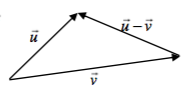
\includegraphics[height=3cm]{th_1}
\end{figure}
\end{frame}



\begin{frame}
  \frametitle{Distancia entre dos puntos}
    \begin{block}{Demostraci\'on}
Por otro lado si se aplica el teorema del coseno al tri\'angulo formado por $\vec u, \vec v $ y $\vec u-\vec v$
\[||\vec u - \vec v||^2 = ||\vec u||^2+||\vec v||^2-2(||\vec u||\cdot ||\vec v|\cos \alpha)\]
 \end{block}

\begin{figure}[h]
    \label{fig:teorema del coseno}
\centering
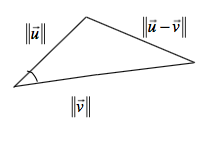
\includegraphics[height=3cm]{th_2}
\end{figure}
\end{frame}

\begin{frame}
  \frametitle{Distancia entre dos puntos}
    \begin{block}{Demostraci\'on}
Si se comparan ambas expresiones se obtiene el resultado:
\[||\vec u - \vec v||^2 = ||\vec u||^2+||\vec v||^2-2(\vec u\cdot \vec v)\]
\[||\vec u - \vec v||^2 = ||\vec u||^2+||\vec v||^2-2(||\vec u||\cdot ||\vec v|\cos \alpha)\]
 \end{block}

\end{frame}

\subsection{\'Angulo entre dos vectores}

\begin{frame}
  \frametitle{\'Angulo entre dos vectores}
  Como se acaba de ver, si $\vec u$ y $\vec v$ forman un \'angulo $\alpha$ entonces se puede definir su producto escalar como $\vec u \cdot \vec v = ||\vec u||\cdot|| \vec v||\cos\alpha$.
    \begin{block}{\'Angulo entre dos vectores}
Se define el \'angulo que forman dos vectores como el valor real $\alpha$:
\[\cos\alpha = \frac{\vec u \cdot \vec v} {||\vec u||\cdot|| \vec v||}\]
 \end{block}
    \begin{block}{Ejercicios}
Encu\'entrese el \'angulo que forman los vectores $(2,3,-1)$ y $(-2,0,3)$
 \end{block}
Sol: $\cos \alpha = -\frac{\sqrt{182}}{26}$
\end{frame}


\begin{frame}
  \frametitle{\'Angulo entre dos vectores}
    \begin{block}{Vectores ortogonales}
Dos vectores son ortogonales si su producto escalar es cero:
\[\vec u \perp \vec v \Leftrightarrow \vec u \cdot \vec v = 0 \Leftrightarrow \alpha = \frac{\pi}{2}\]
 \end{block}
    \begin{block}{Vectores ortonormales}
Dos vectores son ortonormales si son ortogonales y de norma 1.
 \end{block}
Por ejemplo, $(0,1)$ y $(1,0)$ son dos vectores ortonormales. 
\end{frame}


\begin{frame}
  \frametitle{\'Angulo entre dos vectores}
    \begin{block}{Ejercicios}
Encu\'entrese el valor de $a$ para el cual $(a,0,-1,3)$ sea perpendicular a $(1,7,a-1,2a+3)$.
 \end{block}
 Sol: $a=-\frac{5}{3}$
    \begin{block}{Ejercicios}
?`Para que valores de $x$ son ortogonales $(x,-x-8,x,x)$ y $(x,1,-2,1)$?
 \end{block}
Sol: $x=-2$ y $x=4$.
\end{frame}

\subsection{Desigualdad de Cauchy-Schwarz}


\begin{frame}
  \frametitle{Desigualdad de Cauchy-Schwarz}
    \begin{block}{Resultado}
A partir de la expresi\'on:
\[\cos\alpha = \frac{\vec u \cdot \vec v} {||\vec u||\cdot|| \vec v||}\]
Y teniendo en cuenta que el coseno de cualquier \'angulo es siempre menor o igual que 1 se puede obtener:
\[|\vec u\cdot \vec v| \leq ||\vec u||\cdot ||\vec v||\]
  \end{block}
  
 Es decir, que el producto escalar de dos vectores es menor o igual que el producto de sus normas.
\end{frame}


\begin{frame}
  \frametitle{Proyecci\'on ortogonal}
    \begin{block}{Proyecci\'on ortogonal}
La proyecci\'on ortogonal de un vector $\vec v$ sobre otro vector $\vec u$ es un vector paralelo a $\vec u$ tal que sumado a otro perpendicular a $\vec u$ dar\'a $\vec v$ 
  \end{block}
  
\begin{figure}[h]
    \label{fig:ortogonal}
\centering
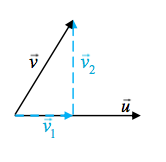
\includegraphics[height=3cm]{ortho}
\end{figure}
\end{frame}


\begin{frame}
  \frametitle{Proyecci\'on ortogonal}
  Se trata de obtener $P_{\vec v} (\vec u) = \vec v_1$ conociendo los vectores $\vec u$ o $\vec v$
    \begin{block}{C\'alculo de la proyecci\'on ortogonal}
\begin{itemize}
\item Se descompone el vector $\vec v = \vec{v_1}+\vec{v_2}$ donde $\vec v_1||\vec u$ i $\vec v_2 \perp \vec u$.
\item $\vec v_1 = \lambda \vec u$
\item $\vec v = \lambda \vec u + \vec{v_2}\Rightarrow \vec v_2 = \vec v - \lambda \vec u$
\item $\vec v_2\cdot \vec u = 0\Rightarrow (\vec v - \lambda \vec u)\cdot \vec u = 0$
\item $\lambda = \frac{\vec v\cdot \vec u}{\vec u\cdot \vec u} = \frac{\vec v\cdot \vec u}{||\vec u||^2}$
\end{itemize}
Por tanto:
\[P_{\vec v} (\vec u) = \vec v_1 = \lambda \vec u = \frac{\vec v\cdot \vec u}{||\vec u||^2} \vec u\]
  \end{block}
  
\end{frame}

\begin{frame}
  \frametitle{Proyecci\'on ortogonal}
    \begin{block}{C\'alculo de la proyecci\'on ortogonal}
Proy\'ectese el vector $\vec v = (1,2)$ sobre $\vec u = (3,1)$.
  \end{block}
  Sol: $P_{\vec v} (\vec u) = \frac{1}{2}(3,1)$.
\end{frame}



\section{Producto vectorial. Producto mixto}

\subsection{Producto vectorial}

\begin{frame}
  \frametitle{Producto vectorial}
    \begin{block}{Producto vectorial}
Sean $\vec u = (u_1,u_2,u_3)$ y $\vec v = (v_1,v_2,v_3)$ dos vectores de $\mathbb R^3$. El producto vectorial de $\vec u$ y $\vec v$ se define como el vector:
\[\vec u \wedge \vec v = (u_2v_3-u_3v_2,u_3v_1-u_1v_3,u_1v_2-u_2v_1)\]
  \end{block}
\end{frame}

\begin{frame}
  \frametitle{Producto vectorial}
    \begin{block}{Resultados}
Si se multiplica escalarmente:
\[\vec u \cdot (\vec u \wedge \vec v )  =0\]
\[\vec v \cdot (\vec u \wedge \vec v )  =0\]
Donde se ve que es perpendicular a $\vec u$ y $\vec v$.
\end{block}
\end{frame}

\begin{frame}
  \frametitle{Producto vectorial}
    \begin{block}{Resultados}
El sentido del producto vectorial es el de indicar\'ia la regla de la mano derecha al llevar el primer vector sobre el segundo por el camino m\'as corto y con m\'odulo el \'area del paralelogramo del determinante dado por $\vec u$ y $\vec v$
\[||\vec u \wedge \vec v|| = ||\vec u ||\cdot h = ||\vec u ||\cdot ||\vec v|| \cdot \sen \alpha \]
  \end{block}
  
  \begin{figure}[h]
    \label{fig:producto vectorial}
\centering
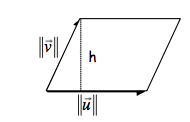
\includegraphics[height=3cm]{pte_vect}
\end{figure}

\end{frame}

\begin{frame}
  \frametitle{Producto vectorial}
    \begin{block}{Producto vectorial como determinante}
\[\vec u \wedge \vec v = (u_2v_3-u_3v_2,u_3v_1-u_1v_3,u_1v_2-u_2v_1)\]
\[\vec u \wedge \vec v = (u_2v_3-u_3v_2)\vec i + (u_3v_1-u_1v_3)\vec j+(u_1v_2-u_2v_1)\vec k\]

\[\vec u \wedge \vec v  =
\left|\begin{array}{ccc}\vec i & \vec j & \vec k \\u_1 & u_2 & u_3 \\v_1 & v_2 & v_3\end{array}\right|
\]

\end{block}
\end{frame}


\begin{frame}
  \frametitle{Producto vectorial}
    \begin{block}{Propiedades}
\begin{itemize}
\item Propiedad anticonmutativa: $\vec u \wedge \vec v = -\vec v \wedge \vec u$
\item Propiedad distributiva:
 \[\vec u \wedge( \vec v+\vec w) = \vec u\wedge \vec v + \vec u \wedge \vec w\]
 \[ ( \vec v+\vec w) \wedge \vec u = \vec v\wedge \vec u + \vec w \wedge \vec u\]
 \item Propiedad asociativa de vectores y escalares:
 \[\alpha\cdot ( \vec u\wedge\vec v) =(\alpha\cdot  \vec u)\wedge\vec v =   \vec u\wedge(\alpha\cdot\vec v) \]
 \item $\vec u \wedge \vec 0 = \vec 0 \wedge \vec u = \vec 0$
 \item $\vec u \wedge \vec u = \vec 0$
\end{itemize}
\end{block}
\end{frame}

\subsection{Producto mixto}

\begin{frame}
  \frametitle{Producte mixto de tres vectores}
    \begin{block}{Producto mixto}
Sean $\vec u = (u_1,u_2,u_3)$, $\vec v = (v_1,v_2,v_3)$ y $\vec w = (w_1,w_2,w_3)$ tres vectores de $\mathbb R^3$ distintos del cero. El producto mixto de $\vec u, \vec v$ y $\vec w$ se define como el vector:
\[\{\vec u, \vec v,\vec w\} = \vec u (\vec v \wedge \vec w)\]
\[\{\vec u, \vec v,\vec w\} = \left|\begin{array}{ccc}u_1 & u_2 & u_3 \\v_1 & v_2 & v_3\\w_1 & w_2 & w_3\end{array}\right|
 \]
  \end{block}
  Si este determinante es cero se puede decir que alguna de las filas es combinaci\'on lineal de las restantes y que por lo tanto uno de los vectores se puede obtener como combinaci\'on lineal de los otros: son coplanarios.
\end{frame}

\begin{frame}
  \frametitle{Producto mixto de tres vectores}
    \begin{block}{Propiedades}
\begin{itemize}
\item $\{\vec u, \vec v,\vec w\} = u_1v_2w_3-u_1v_3w_2+u_2v_3w_1-u_2v_1w_3+u_3v_1w_2-u_3v_2w_1$
\item $\{\vec u, \vec v,\vec w\} = \{\vec v, \vec w,\vec u\} = \{\vec w, \vec u,\vec v\} = -\{\vec v, \vec u,\vec w\} = -\{\vec u, \vec w,\vec v\} = -\{\vec w, \vec v,\vec u\}$
\end{itemize}
\end{block}

  
\end{frame}



\begin{frame}
  \frametitle{Producto mixto de tres vectores}
    \begin{block}{Propietadades}
\begin{itemize}
\item Si los tres vectores son coplanarios, entonces $\{\vec u, \vec v,\vec w\}=0$
\item Si $\{\vec u, \vec v,\vec w\}=0$ entonces o alg\'un vector es $\vec 0$ o los tres vectores son coplanarios
\end{itemize}
\end{block}

  
  \begin{figure}[h]
    \label{fig:producto mixto}
\centering
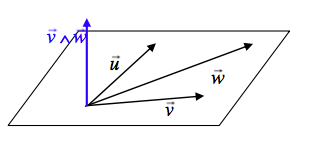
\includegraphics[height=3cm]{pte_mixt}
\end{figure}

\end{frame}


\begin{frame}
  \frametitle{Producto mixto de tres vectores}
    \begin{block}{Propiedades}
\begin{itemize}
\item Geom\'etricamente $\{\vec u, \vec v,\vec w\}$ representa el volumen del paralelep\'ipedo determinado por los tres vectores
\end{itemize}
\end{block}
Pista $\{\vec u, \vec v,\vec w\} = ||\vec u || \cdot ||\vec v \wedge \vec w|| \cos \alpha $, donde $||\vec v \wedge \vec w||$ = \'area de la base y $||\vec u || \cos \alpha$ es la proyecci\'on escalar del vector $\vec u$ sobre la direcci\'on perpendicular a la base, es decir, la altura.
  
  \begin{figure}[h]
    \label{fig:volumen}
\centering
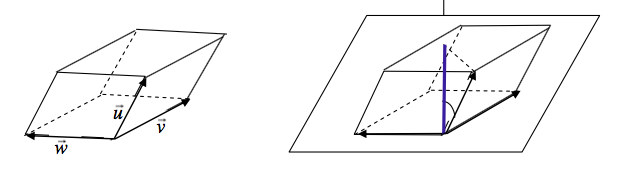
\includegraphics[height=3cm]{volum}
\end{figure}

\end{frame}


\end{document}